% --- IMPORTS ---
\documentclass[leqno]{article}
\usepackage{graphicx}
\usepackage{dsfont}
\usepackage{mathtools}
\usepackage{amssymb}
\usepackage{amsmath}
\usepackage{amsthm}
\usepackage{float}
\usepackage{ragged2e}
\usepackage{tensor}
\usepackage{fancyhdr}
\usepackage{empheq}
\usepackage[most]{tcolorbox}
\usepackage{enumitem}
\usepackage{dirtytalk}
\usepackage{marginnote}
\usepackage{microtype}
\usepackage[
  a4paper,
  left=0.8in,
  right=1in,
  top=1in,
  bottom=0.5in,
  headheight=14pt,
  headsep=0.4in
]{geometry}
\setlength{\parindent}{0cm}
% --- TikZ Packages ---
\usepackage{pgfplots}
\pgfplotsset{compat=1.18}
\usepgfplotslibrary{fillbetween, polar}
\usetikzlibrary{calc, positioning}
\usetikzlibrary{angles, quotes}
\usetikzlibrary{arrows.meta}
\usetikzlibrary{decorations.pathreplacing, decorations.markings}
\usetikzlibrary{patterns}
\usetikzlibrary{intersections}
% --- URL Packages ---
\usepackage[colorlinks=true,linkcolor=red,citecolor=magenta,urlcolor=black]{hyperref}%
\urlstyle{same}
% --- END OF IMPORTS ---

% --- CUSTOM COMMANDS ---
\RenewDocumentCommand{\marks}{o m}{%
  \IfValueTF{#1}%
    {\marginnote{\raggedright\textbf{[#2]}}[#1]}%
    {\marginnote{\raggedright\textbf{[#2]}}}%
}
\newcommand{\vspacerule}[2]{%
  \par\vspace*{#1}%
  \noindent\hrulefill\par
  \vspace*{#2}%
}
\definecolor{scarlet}{RGB}{205, 40, 75}
\newcommand{\questionitem}{%
  \item\phantomsection
  \addcontentsline{toc}{section}{Question \number\value{enumi}}%
}
\renewcommand{\contentsname}{Questions}
% --- END OF CUSTOM COMMANDS ---

% --- HEADER CONFIG ---
\pagestyle{fancy}
\fancyhead{}
\fancyfoot{}
\renewcommand{\headrulewidth}{0.9pt}
\lhead{Complex Roots and Geometry Problems}
\chead{}
\rhead{\href{https://danieljsmith.org}{danieljsmith.org}}
% --- END OF HEADER CONFIG ---

\begin{document}
\vspace*{20pt}
\tableofcontents
\newpage
\begin{enumerate}[
  label=\textbf{\arabic*.},
  leftmargin=*,
  topsep=0pt,
  partopsep=0pt,
  parsep=0pt
]

% ---- Question 1 ----
\questionitem

\begin{figure}[H]
    \centering
\begin{tikzpicture}[scale=1.2]
\coordinate (O) at (0, 0);
\coordinate (A) at (1.6, 1.6);

\draw[thick, -{Stealth[length=3mm]}] (-3.2, 0) -- (3.6, 0) node[right] {$\mathrm{Re}(z)$};
\draw[thick, -{Stealth[length=3mm]}] (0, -3.2) -- (0, 3.6) node[above] {$\mathrm{Im}(z)$};

\draw[thick] ($(A)+(-0.06,0)$) -- ($(A)+(0.06,0)$);
\draw[thick] ($(A)+(0,-0.06)$) -- ($(A)+(0,0.06)$);

\node[below left] at (O) {$O$};
\node[above right] at (A) {$A$};

\end{tikzpicture}
\end{figure}


An Argand diagram with the point $A$ representing a complex number $z_1$ is shown in the diagram. \\
The complex numbers $z_2$, $z_3$ and $z_4$ are $z_1e^{\frac{1}{2}\pi\mathrm{i}}$, $z_1e^{\pi\mathrm{i}}$ and $z_1e^{\frac{3}{2}\pi\mathrm{i}}$ respectively. \\
\begin{enumerate}[label=\textbf{(\alph*)}]
  \item
  \begin{enumerate}[label=(\roman*)]
    \item On a copy of the Argand diagram, mark the points $B$, $C$ and $D$ representing the complex numbers $z_2$, $z_3$ and $z_4$. \marks[-10pt]{2}
    \item Show that $z_1+z_2+z_3+z_4=0$. \marks{2} \\
  \end{enumerate}
  \item Given now that $z_1$, $z_2$, $z_3$ and $z_4$ are roots of the equation $z^4=-16$, find these four roots, giving your answers in the form $a+\mathrm{i}b$, where $a$ and $b$ are real and exact. \marks{4} \\
\end{enumerate}

\vspace*{10pt}

\begin{tcolorbox}[colback=white, colframe=scarlet, title={\textbf{Solution}}, breakable, grow to left by=6mm, grow to right by=10mm]
\begin{enumerate}[label=\textbf{(\alph*)}]
  \item
  \begin{enumerate}[label=(\roman*)]
    \item Multiplying $z_1$ by $e^{i\theta}$ corresponds to rotating $z_1$ by $\theta$ anticlockwise about the origin.

    So \(B\), \(C\) and \(D\) are the images of \(A\) under such rotations of $90^\circ, 180^\circ$ and $270^\circ$ respectively.

    \begin{center}
    \begin{tikzpicture}[scale=1]
      \coordinate (O) at (0,0);
      \coordinate (A) at (1.6,1.6);
      \coordinate (B) at (-1.6,1.6);
      \coordinate (C) at (-1.6,-1.6);
      \coordinate (D) at (1.6,-1.6);

      \draw[thick, -{Stealth[length=3mm]}] (-3.2,0) -- (3.6,0) node[right] {$\mathrm{Re}(z)$};
      \draw[thick, -{Stealth[length=3mm]}] (0,-3.2) -- (0,3.6) node[above] {$\mathrm{Im}(z)$};

      \fill (O) circle (1.2pt);
      \fill (A) circle (1.2pt);
      \fill (B) circle (1.2pt);
      \fill (C) circle (1.2pt);
      \fill (D) circle (1.2pt);

      \node[below left] at (O) {$O$};
      \node[above right] at (A) {$A$};
      \node[above left] at (B) {$B$};
      \node[below left] at (C) {$C$};
      \node[below right] at (D) {$D$};
    \end{tikzpicture}
    \end{center}

    \item
    \begin{align*}
    z_1+z_2+z_3+z_4 &=  z_1+z_1e^{\frac{1}{2}\pi i}+z_1e^{\pi\mathrm{i}}+z_1e^{\frac{3}{2}\pi i}\\
    &=z_1+\mathrm{i}z_1-z_1-\mathrm{i}z_1 \\
    &=z_1(1+\mathrm{i}-1-\mathrm{i}) \\
    &=0
    \end{align*}
    Hence \(z_1+z_2+z_3+z_4=0\).\\

    (Alternatively, use that $1+e^{\frac{1}{2}\pi i}+e^{\pi\mathrm{i}}+e^{\frac{3}{2}\pi i}$ is a geometric sum with common ratio $r = e^{\frac{1}{2}\pi i}$) \\
  \end{enumerate}

  \item Write
  \begin{align*}
        -16&=16e^{\mathrm{i}\pi}\\
           &= 16e^{\mathrm{i}(\pi+2k\pi)}
  \end{align*}

  so the fourth roots are
  \[
  z=2e^{\mathrm{i}\left(\frac{\pi+2k\pi}{4}\right)}
  \qquad k=0,1,2,3
  \]

  Hence
  \begin{align*}
  k=0&:\quad z=2e^{\mathrm{i}\pi/4}
  =2\left(\frac{\sqrt2}{2}+\mathrm{i}\frac{\sqrt2}{2}\right)
  =\sqrt2+\mathrm{i}\sqrt2 \\
  k=1&:\quad z=2e^{3\mathrm{i}\pi/4}
  =2\left(-\frac{\sqrt2}{2}+\mathrm{i}\frac{\sqrt2}{2}\right)
  =-\sqrt2+\mathrm{i}\sqrt2 \\
  k=2&:\quad z=2e^{5\mathrm{i}\pi/4}
  =2\left(-\frac{\sqrt2}{2}-\mathrm{i}\frac{\sqrt2}{2}\right)
  =-\sqrt2-\mathrm{i}\sqrt2 \\
  k=3&:\quad z=2e^{7\mathrm{i}\pi/4}
  =2\left(\frac{\sqrt2}{2}-\mathrm{i}\frac{\sqrt2}{2}\right)
  =\sqrt2-\mathrm{i}\sqrt2
  \end{align*}

  Therefore the four roots are
  \[
  \sqrt2+\mathrm{i}\sqrt2,\quad -\sqrt2+\mathrm{i}\sqrt2,\quad -\sqrt2-\mathrm{i}\sqrt2,\quad \sqrt2-\mathrm{i}\sqrt2
  \]
\end{enumerate}
\end{tcolorbox}


\newpage

% ---- Question 2 ----
\questionitem

The five solutions of the equation $z^5=16+16\sqrt{3}\,\mathrm{i}$ are represented by points on an Argand diagram. \\

These points are the vertices of a regular pentagon $P$ with centre at the origin. \\

\begin{enumerate}
    \item Determine the five complex numbers that represent these vertices, giving your answers in the form $re^{\mathrm{i}\theta}$, where $0\leq \theta<2\pi$. \marks{4} \\

    \item Sketch $P$ on an Argand Diagram, taking care to label each vertex. \marks{2}\\

    \item Show that the area of $P$ can be written $k\sin\frac{2\pi}{5} $ where $k$ is an integer to be determined. \marks{4}

\end{enumerate}

\vspace*{10pt}

\begin{tcolorbox}[colback=white, colframe=scarlet, title={\textbf{Solution}}, breakable, grow to left by=6mm, grow to right by=10mm]
\begin{enumerate}[label=\textbf{(\alph*)}]
  \item Let
\[
w=16+16\sqrt{3}\,\mathrm{i}
\]

First write $w$ in polar form.

Its modulus is
\begin{align*}
|w|
&=\sqrt{16^2+(16\sqrt{3})^2} \\
&=\sqrt{256+768} \\
&=\sqrt{1024} \\
&=32
\end{align*}

Its argument is
\[
\arg(w)=\tan^{-1}\!\left(\frac{16\sqrt{3}}{16}\right)=\tan^{-1}(\sqrt{3})=\frac{\pi}{3}
\]
since $w$ lies in the first quadrant.

So
\[
16+16\sqrt{3}\,\mathrm{i}=32e^{\mathrm{i}\pi/3}
\]

Now solve
\[
z^5=32e^{\mathrm{i}\pi/3}
\]

The fifth roots have modulus
\[
32^{1/5}=2
\]
and arguments
\[
\theta=\frac{\frac{\pi}{3}+2\pi k}{5}=\frac{\pi}{15}+\frac{2\pi k}{5}
\qquad (k=0,1,2,3,4)
\]

Hence the five roots are
\begin{align*}
z&=2e^{\mathrm{i}\pi/15} \\
z&=2e^{\mathrm{i}7\pi/15} \\
z&=2e^{\mathrm{i}13\pi/15} \\
z&=2e^{\mathrm{i}19\pi/15} \\
z&=2e^{\mathrm{i}25\pi/15}=2e^{\mathrm{i}5\pi/3}
\end{align*}

So the five vertices are
\[
2e^{\mathrm{i}\pi/15},\quad
2e^{\mathrm{i}7\pi/15},\quad
2e^{\mathrm{i}13\pi/15},\quad
2e^{\mathrm{i}19\pi/15},\quad
2e^{\mathrm{i}5\pi/3}
\]

  \item Let the vertices in anticlockwise order be
\[
A=2e^{\mathrm{i}\pi/15},\quad
B=2e^{\mathrm{i}7\pi/15},\quad
C=2e^{\mathrm{i}13\pi/15},\quad
D=2e^{\mathrm{i}19\pi/15},\quad
E=2e^{\mathrm{i}5\pi/3}
\]

They all lie on the circle of radius $2$ centred at the origin, with equal angular spacing $\frac{2\pi}{5}$.

\begin{center}
\begin{tikzpicture}
\begin{axis}[
axis lines=middle,
xlabel={$\mathrm{Re}(z)$},
ylabel={$\mathrm{Im}(z)$},
xmin=-3.2, xmax=3.2,
ymin=-3.2, ymax=3.2,
xtick={-2,2},
ytick={-2,2},
width=11cm,
height=11cm,
axis equal image,
clip=false
]
\addplot[black, thick] coordinates {
(1.956,0.416)
(0.209,1.989)
(-1.827,0.813)
(-1.338,-1.486)
(1.000,-1.732)
(1.956,0.416)
};
\addplot[only marks, mark=*] coordinates {
(1.956,0.416)
(0.209,1.989)
(-1.827,0.813)
(-1.338,-1.486)
(1.000,-1.732)
};
\node[anchor=west] at (axis cs:1.956,0.416) {$A$};
\node[anchor=south] at (axis cs:0.209,1.989) {$B$};
\node[anchor=east] at (axis cs:-1.827,0.813) {$C$};
\node[anchor=north east] at (axis cs:-1.338,-1.486) {$D$};
\node[anchor=west] at (axis cs:1.000,-1.732) {$E$};
\node[anchor=north east] at (axis cs:0,0) {$O$};
\end{axis}
\end{tikzpicture}
\end{center}

  \item Join the origin to each vertex. This splits the pentagon into $5$ congruent isosceles triangles.

Each vertex has modulus $2$, so each triangle has two sides of length $2$.

Also, the arguments of adjacent vertices differ by
\[
\frac{2\pi}{5}
\]
so the angle at the origin in each triangle is $\frac{2\pi}{5}$.

Hence the area of one triangle is
\[
\frac12 \times 2 \times 2 \times \sin\frac{2\pi}{5}
=2\sin\frac{2\pi}{5}
\]

Therefore the area of the pentagon $P$ is
\[
5\left(2\sin\frac{2\pi}{5}\right)=10\sin\frac{2\pi}{5}
\]

So it can be written in the form $k\sin\frac{2\pi}{5}$ with
\[
k=10
\]

Hence the area of $P$ is
\[
10\sin\frac{2\pi}{5}
\]
\end{enumerate}
\end{tcolorbox}


\newpage

% ---- Question 3 ----
\questionitem

\begin{enumerate}[label=(\roman*)]
  \item Find the $8$th roots of $-128+128\sqrt{3}\,\mathrm{i}$ in the form $re^{\mathrm{i}\theta}$, where $r>0$ and $0\leq \theta<2\pi$. \marks{5} \\
  \item These $8$th roots are represented in the Argand diagram, in order of increasing $\theta$, by the points $A$, $B$, $C$, $D$, $E$, $F$, $G$, $H$. \\
  Draw the Argand diagram, making clear which point is which. \marks{2} \\
  \item The mid-point of $BD$ is the point $P$ which represents the complex number $w$. \\
  Find, in exact form, the modulus and argument of $w$. \marks{3} \\
  \item $w$ is an $n$th root of a real number $a$, where $n$ is a positive integer. State the least possible value of $n$ and find the corresponding value of $a$. \marks{3} \\
\end{enumerate}

\vspace*{10pt}

\begin{tcolorbox}[colback=white, colframe=scarlet, title={\textbf{Solution}}, breakable, grow to left by=6mm, grow to right by=10mm]
\begin{enumerate}[label=\textbf{(\roman*)}]
\item Let
\[
z=-128+128\sqrt{3}\,\mathrm{i}
\]

Its modulus is
\begin{align*}
|z|
&=\sqrt{(-128)^2+(128\sqrt{3})^2} \\
&=128\sqrt{1+3} \\
&=256
\end{align*}

Also,
\[
\tan \theta=\frac{128\sqrt{3}}{-128}=-\sqrt{3}
\]
Since \(z\) lies in the second quadrant, its argument is
\[
\theta=\frac{2\pi}{3}
\]

So
\[
-128+128\sqrt{3}\,\mathrm{i}=256e^{\mathrm{i}2\pi/3}
\]

If \(z_k\) is an 8th root, then
\[
z_k^8=256e^{\mathrm{i}2\pi/3}
\]
Hence the modulus of each root is
\[
256^{1/8}=2
\]
and the arguments are
\begin{align*}
\frac{\frac{2\pi}{3}+2k\pi}{8}
&=\frac{\pi}{12}+\frac{k\pi}{4},
\qquad k=0,1,\ldots,7
\end{align*}

Therefore the 8th roots are
\[
z_k=2e^{\mathrm{i}\left(\pi/12+k\pi/4\right)},
\qquad k=0,1,\ldots,7
\]

\item In increasing order of argument, the points are
\[
A:\frac{\pi}{12},\quad
B:\frac{\pi}{3},\quad
C:\frac{7\pi}{12},\quad
D:\frac{5\pi}{6},\quad
E:\frac{13\pi}{12},\quad
F:\frac{4\pi}{3},\quad
G:\frac{19\pi}{12},\quad
H:\frac{11\pi}{6}
\]

All eight points lie on the circle \(|z|=2\).

\begin{center}
\begin{tikzpicture}
\begin{axis}[
axis lines=middle,
xlabel={$\mathrm{Re}(z)$},
ylabel={$\mathrm{Im}(z)$},
xmin=-3.5, xmax=3.5,
ymin=-3.5, ymax=3.5,
width=12cm, height=12cm,
axis equal image,
ticks=none,
clip=false
]
\addplot[only marks, mark=*, mark size=1.6pt] coordinates {
(1.9319,0.5176)
(1,1.7321)
(-0.5176,1.9319)
(-1.7321,1)
(-1.9319,-0.5176)
(-1,-1.7321)
(0.5176,-1.9319)
(1.7321,-1)
};
\node[anchor=west] at (axis cs:1.9319,0.5176) {$A$};
\node[anchor=west] at (axis cs:1,1.7321) {$B$};
\node[anchor=south east] at (axis cs:-0.5176,1.9319) {$C$};
\node[anchor=east] at (axis cs:-1.7321,1) {$D$};
\node[anchor=east] at (axis cs:-1.9319,-0.5176) {$E$};
\node[anchor=east] at (axis cs:-1,-1.7321) {$F$};
\node[anchor=north east] at (axis cs:0.5176,-1.9319) {$G$};
\node[anchor=west] at (axis cs:1.7321,-1) {$H$};
\end{axis}
\end{tikzpicture}
\end{center}

\item The complex numbers represented by \(B\) and \(D\) are
\[
2e^{\mathrm{i}\pi/3}
\quad\text{and}\quad
2e^{\mathrm{i}5\pi/6}
\]
Since \(P\) is the midpoint of \(BD\), the complex number \(w\) is
\begin{align*}
w
&=\frac{2e^{\mathrm{i}\pi/3}+2e^{\mathrm{i}5\pi/6}}{2} \\
&=e^{\mathrm{i}\pi/3}+e^{\mathrm{i}5\pi/6} \\
&=e^{\mathrm{i}7\pi/12}\left(e^{-\mathrm{i}\pi/4}+e^{\mathrm{i}\pi/4}\right) \\
&=e^{\mathrm{i}7\pi/12}\left(2\cos\frac{\pi}{4}\right) \\
&=\sqrt{2}\,e^{\mathrm{i}7\pi/12}
\end{align*}

So the modulus and argument of \(w\) are
\[
|w|=\sqrt{2},
\qquad
\arg(w)=\frac{7\pi}{12}
\]

\item Since
\[
w=\sqrt{2}\,e^{\mathrm{i}7\pi/12}
\]
we have
\[
w^n=(\sqrt{2})^n e^{\mathrm{i}7n\pi/12}
\]

For \(w^n\) to be real, its argument must be a multiple of \(\pi\), so
\[
\frac{7n\pi}{12}=m\pi
\]
for some integer \(m\). Hence
\[
\frac{7n}{12}\in\mathbb{Z}
\]
As 7 and 12 have no common factor, the least possible value is
\[
n=12
\]

Then
\begin{align*}
a
&=w^{12} \\
&=(\sqrt{2})^{12}e^{\mathrm{i}7\pi} \\
&=2^6(-1) \\
&=-64
\end{align*}

So the least possible value of \(n\) is \(12\), and the corresponding value of \(a\) is \(-64\).
\end{enumerate}
\end{tcolorbox}


\newpage

% ---- Question 4 ----
\questionitem

Given that $z_1=7-\mathrm{i}$ and $z_2=\dfrac{z_1}{1-\mathrm{i}}$, \\
\begin{enumerate}[label=\textbf{(\alph*)}]
  \item find $z_2$ in the form $a+b\mathrm{i}$, where $a$ and $b$ are real. \marks{2} \\
  \item Show on an Argand diagram the point $P$ representing $z_1$ and the point $Q$ representing $z_2$. \marks{2} \\
  \item Given that $O$ is the origin, show that $\angle OQP=\dfrac{\pi}{2}$. \marks{2} \\
\end{enumerate}
The circle passing through the points $O$, $P$ and $Q$ has centre $C$. Find \\
\begin{enumerate}[label=\textbf{(\alph*)}, resume]
  \item the complex number represented by $C$. \marks{2} \\
  \item the exact value of the radius of the circle. \marks{2} \\
\end{enumerate}

\vspace*{10pt}

\begin{tcolorbox}[colback=white, colframe=scarlet, title={\textbf{Solution}}, breakable, grow to left by=6mm, grow to right by=10mm]
\begin{enumerate}[label=\textbf{(\alph*)}]
  \item Rationalise the denominator:
  \begin{align*}
  z_2&=\frac{7-\mathrm{i}}{1-\mathrm{i}}\cdot\frac{1+\mathrm{i}}{1+\mathrm{i}}\\
     &=\frac{(7-\mathrm{i})(1+\mathrm{i})}{(1-\mathrm{i})(1+\mathrm{i})}\\
     &=\frac{7+7\mathrm{i}-\mathrm{i}-\mathrm{i}^2}{1-\mathrm{i}^2}\\
     &=\frac{7+6\mathrm{i}+1}{1+1}\\
     &=\frac{8+6\mathrm{i}}{2}\\
     &=4+3\mathrm{i}
  \end{align*}
  Hence,
  \[
  z_2=4+3\mathrm{i}
  \]
  
  \item On an Argand diagram, the complex number $x+y\mathrm{i}$ is represented by the point $(x,y)$.

  So
  \[
  z_1=7-\mathrm{i}\;\Rightarrow\;P(7,-1),\qquad z_2=4+3\mathrm{i}\;\Rightarrow\;Q(4,3)
  \]

  \begin{center}
  \begin{tikzpicture}
  \begin{axis}[
    axis lines=middle,
    xmin=-0.5, xmax=9,
    ymin=-2, ymax=5,
    width=10cm, height=7.5cm,
    xlabel={$\mathrm{Re}(z)$},
    ylabel={$\mathrm{Im}(z)$},
    xtick={4,7},
    ytick={-1,3},
    enlargelimits=false
  ]
  \addplot[only marks, mark=*, mark size=2.2pt] coordinates {(7,-1) (4,3)};
  \node at (axis cs:7.25,-1.2) {$P$};
  \node at (axis cs:4.25,3.2) {$Q$};
  \end{axis}
  \end{tikzpicture}
  \end{center}

  \item Using the coordinates from part (b),
  \[
  O=(0,0),\quad P=(7,-1),\quad Q=(4,3)
  \]

  Take the vectors from $Q$:
  \[
  \overrightarrow{QO}=(-4,-3),\qquad \overrightarrow{QP}=(3,-4)
  \]

  Their scalar product is
  \begin{align*}
  \overrightarrow{QO}\cdot\overrightarrow{QP}
  &=(-4)(3)+(-3)(-4)\\
  &=-12+12\\
  &=0
  \end{align*}

  So $\overrightarrow{QO}$ is perpendicular to $\overrightarrow{QP}$, which means
  \[
  \angle OQP=\frac{\pi}{2}
  \]

  \item Since $\angle OQP=\dfrac{\pi}{2}$, the side $OP$ is a diameter of the circle through $O$, $P$ and $Q$.

  Therefore the centre $C$ is the midpoint of $O(0,0)$ and $P(7,-1)$:
  \begin{align*}
  C&=\left(\frac{0+7}{2},\frac{0+(-1)}{2}\right)\\
   &=\left(\frac72,-\frac12\right)
  \end{align*}

  So the complex number represented by $C$ is
  \[
  \frac72-\frac12\mathrm{i}
  \]

  \item The diameter is $OP$, so first find its length:
  \begin{align*}
  OP&=\sqrt{(7-0)^2+(-1-0)^2}\\
    &=\sqrt{49+1}\\
    &=\sqrt{50}\\
    &=5\sqrt2
  \end{align*}

  Hence the radius of the circle is
  \[
  \frac{1}{2}OP=\frac{5\sqrt2}{2}
  \]

  So the exact radius is $\dfrac{5\sqrt2}{2}$.
\end{enumerate}
\end{tcolorbox}


\newpage

% ---- Question 5 ----
\questionitem

\begin{figure}[H]
    \centering
\begin{tikzpicture}[scale=1.5]
\def\rad{2}
\coordinate (O) at (0,0);
\coordinate (A) at (\rad,0);
\coordinate (B) at (120:\rad);
\coordinate (C) at (240:\rad);
\coordinate (P) at ({3*\rad},0);
\coordinate (Q) at ({1.5*\rad},{sqrt(3)*\rad/2});
\coordinate (R) at ({1.5*\rad},{-sqrt(3)*\rad/2});
\draw[-{Stealth[length=3mm]}, thick] ({-0.9*\rad},0) -- ({3.35*\rad},0) node[right] {$\mathrm{Re}(z)$};
\draw[-{Stealth[length=3mm]}, thick] (0,{-1.2*\rad}) -- (0,{1.2*\rad}) node[above] {$\mathrm{Im}(z)$};
\draw[thick] (A) -- (B) -- (C) -- cycle;
\draw[thick] (P) -- (Q) -- (R) -- cycle;
\node[below] at (A) {$A$};
\node[above left] at (B) {$B$};
\node[below left] at (C) {$C$};
\node[below] at (P) {$P$};
\node[above right] at (Q) {$Q$};
\node[below right] at (R) {$R$};
\node[below left] at (O) {$O$};
\end{tikzpicture}
\end{figure}


The cube roots of unity are represented on the Argand diagram below by the points $A$, $B$ and $C$. \\

The complex numbers represented by $P$, $Q$ and $R$ are obtained by adding $2$ to the complex numbers represented by $A$, $B$ and $C$ respectively. \\

Determine a degree $6$ polynomial equation with integer coefficients whose roots are the complex numbers represented by the points $A$, $B$, $C$, $P$, $Q$ and $R$. \marks{5}

\vspace*{15pt}

\begin{tcolorbox}[colback=white, colframe=scarlet, title={\textbf{Solution}}, breakable, grow to left by=6mm, grow to right by=10mm]
Let the required polynomial have variable \(z\).

The points \(A,B,C\) represent the cube roots of unity, so their complex numbers satisfy
\[
z^3=1
\]
Hence \(A,B,C\) are the roots of
\[
z^3-1=0
\]

Now \(P,Q,R\) are obtained by adding \(2\) to the complex numbers at \(A,B,C\).

So if \(z\) represents one of \(P,Q,R\), then \(z-2\) is a cube root of unity. Therefore
\[
(z-2)^3=1
\]
so
\[
(z-2)^3-1=0
\]

Expanding:
\begin{align*}
(z-2)^3-1&=(z^3-6z^2+12z-8)-1 \\
&=z^3-6z^2+12z-9
\end{align*}

So \(P,Q,R\) are the roots of
\[
z^3-6z^2+12z-9=0
\]

Therefore a degree \(6\) polynomial with roots \(A,B,C,P,Q,R\) is
\[
(z^3-1)(z^3-6z^2+12z-9)=0
\]

Now expand:
\begin{align*}
(z^3-1)(z^3-6z^2+12z-9)
&=z^3(z^3-6z^2+12z-9)-(z^3-6z^2+12z-9) \\
&=z^6-6z^5+12z^4-9z^3-z^3+6z^2-12z+9 \\
&=z^6-6z^5+12z^4-10z^3+6z^2-12z+9
\end{align*}

Hence the required polynomial equation is
\[
z^6-6z^5+12z^4-10z^3+6z^2-12z+9=0
\]
\end{tcolorbox}


\newpage

% ---- Question 6 ----
\questionitem

In an Argand diagram, the points $A$, $B$ and $C$ are the vertices of an equilateral triangle with centre $G$. The point $G$ represents the complex number $1-2\mathrm{i}$, and the point $A$ represents the complex number $5+2\mathrm{i}$. \\
\begin{enumerate}[label=\textbf{(\alph*)}]
  \item Find the complex numbers represented by the points $B$ and $C$, giving your answers in the form $x+\mathrm{i}y$, where $x$ and $y$ are real and exact. \marks{6} \\
\end{enumerate}
The points $D$, $E$ and $F$ are the centroids of triangles $GBC$, $GCA$ and $GAB$ respectively. \\
\begin{enumerate}[label=\textbf{(\alph*)}, resume]
  \item Find the exact area of triangle $DEF$. \marks{4} \\
\end{enumerate}

\vspace*{10pt}

\begin{tcolorbox}[colback=white, colframe=scarlet, title={\textbf{Solution}}, breakable, grow to left by=6mm, grow to right by=10mm]
\begin{enumerate}[label=\textbf{(\alph*)}]
  \item Let
  \[
  z_G=1-2i,\qquad z_A=5+2i
  \]
  Then the vector from \(G\) to \(A\) is
  \[
  z_A-z_G=(5+2i)-(1-2i)=4+4i
  \]

  In an equilateral triangle, the vectors from the centre to the three vertices are \(120^\circ\) apart. So the vectors from \(G\) to \(B\) and \(C\) are obtained by rotating \(4+4i\) through \(\pm 120^\circ\).

  Take \(B\) to be the \(+120^\circ\) rotation. Then
  \[
  z_B-z_G=(4+4i)\left(-\frac12+\frac{\sqrt3}{2}i\right)
  \]
  Expanding,
  \begin{align*}
  z_B-z_G
  &=4\left(-\frac12\right)+4\left(\frac{\sqrt3}{2}i\right)+4i\left(-\frac12\right)+4i\left(\frac{\sqrt3}{2}i\right) \\
  &=-2+2\sqrt3\,i-2i+2\sqrt3\,i^2 \\
  &=-2-2\sqrt3+(2\sqrt3-2)i
  \end{align*}
  Hence
  \begin{align*}
  z_B&=z_G+(z_B-z_G) \\
  &=(1-2i)+\bigl[-2-2\sqrt3+(2\sqrt3-2)i\bigr] \\
  &=-1-2\sqrt3+(2\sqrt3-4)i
  \end{align*}

  Now take \(C\) to be the \(-120^\circ\) rotation. Then
  \[
  z_C-z_G=(4+4i)\left(-\frac12-\frac{\sqrt3}{2}i\right)
  \]
  Expanding,
  \begin{align*}
  z_C-z_G
  &=4\left(-\frac12\right)+4\left(-\frac{\sqrt3}{2}i\right)+4i\left(-\frac12\right)+4i\left(-\frac{\sqrt3}{2}i\right) \\
  &=-2-2\sqrt3\,i-2i-2\sqrt3\,i^2 \\
  &=-2+2\sqrt3-(2+2\sqrt3)i
  \end{align*}
  Hence
  \begin{align*}
  z_C&=z_G+(z_C-z_G) \\
  &=(1-2i)+\bigl[-2+2\sqrt3-(2+2\sqrt3)i\bigr] \\
  &=-1+2\sqrt3-(4+2\sqrt3)i
  \end{align*}

  Therefore
  \[
  B=-1-2\sqrt3+(2\sqrt3-4)i,\qquad
  C=-1+2\sqrt3-(4+2\sqrt3)i
  \]
  with \(B\) and \(C\) interchangeable.

  \item Since \(G\) is the centre of the equilateral triangle \(ABC\), it is also the centroid of \(ABC\). Therefore
  \[
  z_G=\frac{z_A+z_B+z_C}{3}
  \]
  so
  \[
  z_B+z_C=3z_G-z_A
  \]

  The centroid of triangle \(GBC\) is \(D\), so
  \begin{align*}
  z_D&=\frac{z_G+z_B+z_C}{3} \\
  &=\frac{z_G+(3z_G-z_A)}{3} \\
  &=\frac{4z_G-z_A}{3}
  \end{align*}
  Similarly,
  \[
  z_E=\frac{4z_G-z_B}{3},\qquad z_F=\frac{4z_G-z_C}{3}
  \]

  Now compare these with \(z_G\):
  \begin{align*}
  z_D-z_G&=\frac{4z_G-z_A}{3}-z_G=\frac{z_G-z_A}{3}=-\frac13(z_A-z_G) \\
  z_E-z_G&=-\frac13(z_B-z_G) \\
  z_F-z_G&=-\frac13(z_C-z_G)
  \end{align*}

  So triangle \(DEF\) is similar to triangle \(ABC\), with all lengths scaled by a factor of \(\frac13\). Hence the area scale factor is
  \[
  \left(\frac13\right)^2=\frac19
  \]

  Next, find the area of \(ABC\)

  First,
  \[
  GA=|z_A-z_G|=|4+4i|=\sqrt{4^2+4^2}=4\sqrt2
  \]

  Since \(G\) is the centre of the equilateral triangle, the three angles at \(G\) are equal and sum to \(360^\circ\), so
  \[
  \angle AGB=120^\circ
  \]

  Also,
  \[
  GA=GB=GC=4\sqrt2
  \]

  Hence
  \begin{align*}
  \text{Area of } \triangle AGB
  &=\frac12(GA)(GB)\sin 120^\circ \\
  &=\frac12(4\sqrt2)(4\sqrt2)\cdot \frac{\sqrt3}{2} \\
  &=16\cdot \frac{\sqrt3}{2} \\
  &=8\sqrt3
  \end{align*}

  The triangle \(ABC\) is made up of the three congruent triangles \(AGB\), \(BGC\) and \(CGA\), so
  \[
  \text{Area of }ABC=3(8\sqrt3)=24\sqrt3
  \]

  Therefore
  \begin{align*}
  \text{Area of }DEF
  &=\frac19 \times 24\sqrt3 \\
  &=\frac{8\sqrt3}{3}
  \end{align*}

  The exact area of triangle \(DEF\) is
  \[
  \frac{8\sqrt3}{3}
  \]
\end{enumerate}
\end{tcolorbox}


\newpage

% ---- Question 7 ----
\questionitem

\begin{figure}[H]
    \centering
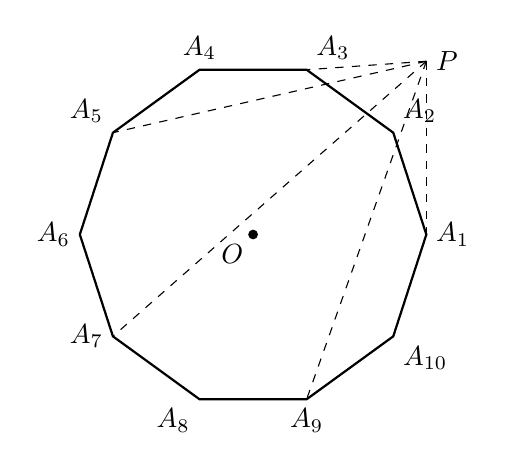
\begin{tikzpicture}[scale=2.2]
\def\R{1}
\pgfmathsetmacro{\step}{360/10}

\coordinate (O) at (0,0);
\coordinate (P) at (1,1);

\foreach \k/\name in {0/A1,1/A2,2/A3,3/A4,4/A5,5/A6,6/A7,7/A8,8/A9,9/A10}{
  \coordinate (\name) at ({\k*\step}:\R);
}

\draw[thick] (A1) -- (A2) -- (A3) -- (A4) -- (A5) -- (A6) -- (A7) -- (A8) -- (A9) -- (A10) -- cycle;

\foreach \Q in {A1,A3,A5,A7,A9}{
  \draw[dashed] (P) -- (\Q);
}

\fill (O) circle[radius=0.8pt];
\node[below left] at (O) {$O$};
\node[right] at (P) {$P$};
\node[right] at (A1) {$A_1$};
\node[above right] at (A2) {$A_2$};
\node[above right] at (A3) {$A_3$};
\node[above] at (A4) {$A_4$};
\node[above left] at (A5) {$A_5$};
\node[left] at (A6) {$A_6$};
\node[left] at (A7) {$A_7$};
\node[below left] at (A8) {$A_8$};
\node[below] at (A9) {$A_9$};
\node[below right] at (A10) {$A_{10}$};
\end{tikzpicture}
\end{figure}


\begin{enumerate}[label=\textbf{(\alph*)}]
  \item Using the identity $zz^*=|z|^2$, or otherwise, show that if $w$ is any root of unity then
  \[
  |w-(1+\mathrm{i})|^2=3-(1-\mathrm{i})w-(1+\mathrm{i})w^*
  \]
  \marks[-20pt]{3}
\end{enumerate}
The diagram shows a regular decagon $A_1A_2\ldots A_{10}$ whose vertices all lie on the unit circle with centre at the origin $O$ and $A_1$ at $(1,0)$. The point $P$ lies in the same plane as the decagon and has coordinates $(1,1)$. \\

\begin{enumerate}[label=\textbf{(\alph*)}, resume]
  \item Using the result from part (a), find
\[
\sum_{r=1}^{5}(PA_{2r-1})^2
\]\marks[-20pt]{4}
\end{enumerate}

\vspace*{10pt}

\begin{tcolorbox}[colback=white, colframe=scarlet, title={\textbf{Solution}}, breakable, grow to left by=6mm, grow to right by=10mm]
\begin{enumerate}[label=\textbf{(\alph*)}]
  \item Using
\[
|z|^2=zz^*
\]
we have
\begin{align*}
|w-(1+\mathrm{i})|^2
&=\bigl(w-(1+\mathrm{i})\bigr)\bigl(w^*-(1-\mathrm{i})\bigr) \\
&=ww^*-(1-\mathrm{i})w-(1+\mathrm{i})w^*+(1+\mathrm{i})(1-\mathrm{i})
\end{align*}

Now $w$ is a root of unity, so $|w|=1$. Hence
\[
ww^*=|w|^2=1
\]
Also,
\[
(1+\mathrm{i})(1-\mathrm{i})=1-\mathrm{i}^2=2
\]
So
\begin{align*}
|w-(1+\mathrm{i})|^2
&=1-(1-\mathrm{i})w-(1+\mathrm{i})w^*+2 \\
&=3-(1-\mathrm{i})w-(1+\mathrm{i})w^*
\end{align*}

Therefore
\[
|w-(1+\mathrm{i})|^2 = 3-(1-\mathrm{i})w-(1+\mathrm{i})w^*
\]

  \item Let the complex number representing $A_{2r-1}$ be $w_r$.

Since the decagon is regular and $A_1=(1,0)$, the odd-numbered vertices are at arguments
\[
0,\ \frac{2\pi}{5},\ \frac{4\pi}{5},\ \frac{6\pi}{5},\ \frac{8\pi}{5}
\]
so
\[
w_r=e^{2\pi \mathrm{i}(r-1)/5}\qquad (r=1,2,3,4,5)
\]
These are exactly the 5th roots of unity.

Also, the point $P=(1,1)$ corresponds to the complex number $1+\mathrm{i}$. Therefore
\[
PA_{2r-1}=|w_r-(1+\mathrm{i})|
\]
and so
\[
(PA_{2r-1})^2=|w_r-(1+\mathrm{i})|^2
\]

Using the result from part (a),
\[
(PA_{2r-1})^2=3-(1-\mathrm{i})w_r-(1+\mathrm{i})w_r^*
\]

Now sum for $r=1$ to $5$:
\begin{align*}
\sum_{r=1}^{5} (PA_{2r-1})^2
&=\sum_{r=1}^{5}\left(3-(1-\mathrm{i})w_r-(1+\mathrm{i})w_r^*\right) \\
&=15-(1-\mathrm{i})\sum_{r=1}^{5} w_r-(1+\mathrm{i})\sum_{r=1}^{5} w_r^*
\end{align*}

Since $w_1,w_2,w_3,w_4,w_5$ are the 5th roots of unity,
\[
\sum_{r=1}^{5} w_r=0
\]
Taking complex conjugates gives
\[
\sum_{r=1}^{5} w_r^*=0
\]

Hence
\[
\sum_{r=1}^{5} (PA_{2r-1})^2=15
\]

\end{enumerate}
\end{tcolorbox}


\newpage

% ---- Question 8 ----
\questionitem

You are given the complex number $\alpha=\cos \frac{3\pi}{5}+\mathrm{i}\sin \frac{3\pi}{5}$ and the equation $z^5=-1$. \\
\begin{enumerate}[label=\textbf{(\alph*)}]
  \item Show that $\alpha$ is a root of the equation. \marks{2} \\
  \item Write down the other four roots of the equation. \marks{1} \\
  \item Show that
  \[
  \alpha^4-\alpha^3+\alpha^2-\alpha+1=0
  \]
  \marks[-20pt]{2}
  \item Hence show that
  \[
  \left(\alpha+\frac{1}{\alpha}\right)^2-\left(\alpha+\frac{1}{\alpha}\right)-1=0
  \]
  \marks[-30pt]{3}
  \item Hence determine the value of $\cos \frac{3\pi}{5}$ in the form $a+b\sqrt{c}$, where $a$, $b$ and $c$ are rational numbers to be found. \marks{4} \\
\end{enumerate}

\vspace*{10pt}

\begin{tcolorbox}[colback=white, colframe=scarlet, title={\textbf{Solution}}, breakable, grow to left by=6mm, grow to right by=10mm]
\begin{enumerate}[label=\textbf{(\alph*)}]
  \item We have
\[
\alpha=\cos\frac{3\pi}{5}+\mathrm{i}\sin\frac{3\pi}{5}
\]

Using De Moivre's theorem,
\begin{align*}
\alpha^5
&=\cos\left(5\cdot\frac{3\pi}{5}\right)+\mathrm{i}\sin\left(5\cdot\frac{3\pi}{5}\right) \\
&=\cos 3\pi+\mathrm{i}\sin 3\pi \\
&=-1+0\mathrm{i} \\
&=-1
\end{align*}

So $\alpha$ satisfies $z^5=-1$, and hence $\alpha$ is a root of the equation.

  \item Since
\[
-1=\cos\bigl((2k+1)\pi\bigr)+\mathrm{i}\sin\bigl((2k+1)\pi\bigr)
\]
the five roots are
\[
z=\cos\frac{(2k+1)\pi}{5}+\mathrm{i}\sin\frac{(2k+1)\pi}{5}
\qquad (k=0,1,2,3,4)
\]

Given that $\alpha=\cos\frac{3\pi}{5}+\mathrm{i}\sin\frac{3\pi}{5}$, the other four roots are
\[
\cos\frac{\pi}{5}+\mathrm{i}\sin\frac{\pi}{5},\quad
\cos\pi+\mathrm{i}\sin\pi,\quad
\cos\frac{7\pi}{5}+\mathrm{i}\sin\frac{7\pi}{5},\quad
\cos\frac{9\pi}{5}+\mathrm{i}\sin\frac{9\pi}{5}
\]

  \item From part (a), $\alpha^5=-1$, so
\[
\alpha^5+1=0
\]

Divide $x^5+1$ by $x+1$ to obtain the factorisation
\[
x^5+1=(x+1)(x^4-x^3+x^2-x+1)
\]

Hence
\[
(\alpha+1)(\alpha^4-\alpha^3+\alpha^2-\alpha+1)=0
\]

But $\alpha\ne -1$, since $\alpha=\cos\frac{3\pi}{5}+\mathrm{i}\sin\frac{3\pi}{5}$ and $\sin\frac{3\pi}{5}\ne 0$.

Therefore
\[
\alpha^4-\alpha^3+\alpha^2-\alpha+1=0
\]

  \item Since $\alpha\neq 0$, divide the result from part (c) by $\alpha^2$:
\begin{align*}
\frac{\alpha^4}{\alpha^2}-\frac{\alpha^3}{\alpha^2}+\frac{\alpha^2}{\alpha^2}-\frac{\alpha}{\alpha^2}+\frac{1}{\alpha^2}&=0 \\
\alpha^2-\alpha+1-\frac{1}{\alpha}+\frac{1}{\alpha^2}&=0
\end{align*}

Let
\[
t=\alpha+\frac{1}{\alpha}
\]

Then
\begin{align*}
t^2
&=\left(\alpha+\frac{1}{\alpha}\right)^2 \\
&=\alpha^2+2+\frac{1}{\alpha^2}
\end{align*}
so
\[
\alpha^2+\frac{1}{\alpha^2}=t^2-2
\]

Also,
\[
\alpha+\frac{1}{\alpha}=t
\]

Substituting into
\[
\alpha^2-\alpha+1-\frac{1}{\alpha}+\frac{1}{\alpha^2}=0
\]
gives
\begin{align*}
\left(\alpha^2+\frac{1}{\alpha^2}\right)-\left(\alpha+\frac{1}{\alpha}\right)+1&=0 \\
(t^2-2)-t+1&=0 \\
t^2-t-1&=0
\end{align*}

Therefore,
\[
\left(\alpha+\frac{1}{\alpha}\right)^2-\left(\alpha+\frac{1}{\alpha}\right)-1=0
\]

  \item From part (d), let
\[
t=\alpha+\frac{1}{\alpha}
\]
so that
\[
t^2-t-1=0
\]

Solving this quadratic,
\[
t=\frac{1\pm\sqrt{5}}{2}
\]

Now
\[
\alpha=\cos\frac{3\pi}{5}+\mathrm{i}\sin\frac{3\pi}{5}
\]
and since $|\alpha|=1$,
\[
\frac{1}{\alpha}=\cos\frac{3\pi}{5}-\mathrm{i}\sin\frac{3\pi}{5}
\]

Hence
\begin{align*}
\alpha+\frac{1}{\alpha}
&=\left(\cos\frac{3\pi}{5}+\mathrm{i}\sin\frac{3\pi}{5}\right)+\left(\cos\frac{3\pi}{5}-\mathrm{i}\sin\frac{3\pi}{5}\right) \\
&=2\cos\frac{3\pi}{5}
\end{align*}

So
\[
2\cos\frac{3\pi}{5}=\frac{1\pm\sqrt{5}}{2}
\]

Therefore
\[
\cos\frac{3\pi}{5}=\frac{1\pm\sqrt{5}}{4}
\]

Since $\frac{3\pi}{5}=108^\circ$ is in quadrant II, $\cos\frac{3\pi}{5}<0$, so we take the negative value:

\[
\cos\frac{3\pi}{5}=\frac{1-\sqrt{5}}{4}
\]

So the required value is
\[
\cos\frac{3\pi}{5}=\frac{1-\sqrt{5}}{4}
\]
\end{enumerate}
\end{tcolorbox}


\newpage

% ---- Question 9 ----
\questionitem

The points representing the complex numbers $z_1=6+11\mathrm{i}$ and $z_2=-8-3\mathrm{i}$ are opposite vertices of a regular octagon, $K$, in the complex plane. \\
The centre of $K$ represents the complex number $\alpha$. \\
\begin{enumerate}[label=\textbf{(\alph*)}]
  \item Show that $\alpha=-1+4\mathrm{i}$. \marks{2} \\
\end{enumerate}
Given that
\[
\beta=\frac{1-\mathrm{i}}{14}
\]
\begin{enumerate}[label=\textbf{(\alph*)}, resume]
  \item Show that
  \[
  \beta(z_1-\alpha)=1
  \]
  \marks[-20pt]{2}
\end{enumerate}
The vertices of $K$ are given by the roots of the equation
\[
(\beta(z-\alpha))^8=1
\]
\begin{enumerate}[label=\textbf{(\alph*)}, resume]
  \item
  \begin{enumerate}[label=(\roman*)]
    \item Write down the roots of the equation $w^8=1$ in the form $re^{\mathrm{i}\theta}$. \marks{1}
    \item Hence, or otherwise, determine the positions of the other six vertices of $K$, giving your answers as complex numbers in Cartesian form. \marks{4} \\
  \end{enumerate}
\end{enumerate}

\vspace*{10pt}

\begin{tcolorbox}[colback=white, colframe=scarlet, title={\textbf{Solution}}, breakable, grow to left by=6mm, grow to right by=10mm]
\begin{enumerate}[label=\textbf{(\alph*)}]
  \item Since $z_1$ and $z_2$ are opposite vertices of the regular octagon, the centre is the midpoint of the line joining them.

\[
\alpha=\frac{z_1+z_2}{2}
=\frac{(6+11\mathrm{i})+(-8-3\mathrm{i})}{2}
\]

\[
\alpha=\frac{-2+8\mathrm{i}}{2}=-1+4\mathrm{i}
\]

So $\alpha=-1+4\mathrm{i}$.

  \item First find $z_1-\alpha$:

\[
z_1-\alpha=(6+11\mathrm{i})-(-1+4\mathrm{i})
=7+7\mathrm{i}
=7(1+\mathrm{i})
\]

Now multiply by $\beta$:

\[
\beta(z_1-\alpha)=\frac{1-\mathrm{i}}{14}\cdot 7(1+\mathrm{i})
=\frac{(1-\mathrm{i})(1+\mathrm{i})}{2}
\]

Using $(1-\mathrm{i})(1+\mathrm{i})=1-\mathrm{i}^2=2$,

\[
\beta(z_1-\alpha)=\frac{2}{2}=1
\]

Hence $\beta(z_1-\alpha)=1$.

  \item 
  \begin{enumerate}[label=(\roman*)]
    \item The roots of $w^8=1$ are the eighth roots of unity:

\[
w=e^{\mathrm{i}k\pi/4},\qquad k=0,1,2,3,4,5,6,7
\]

So in the form $re^{\mathrm{i}\theta}$, we have $r=1$ and $\theta=\dfrac{k\pi}{4}$.

    \item From
\[
(\beta(z-\alpha))^8=1
\]
let
\[
w=\beta(z-\alpha)
\]
Then $w^8=1$, so

\[
z-\alpha=\frac{w}{\beta}
\qquad\Rightarrow\qquad
z=\alpha+\frac{w}{\beta}
\]

Now
\[
\frac{1}{\beta}=\frac{14}{1-\mathrm{i}}
=\frac{14(1+\mathrm{i})}{(1-\mathrm{i})(1+\mathrm{i})}
=\frac{14(1+\mathrm{i})}{2}
=7(1+\mathrm{i})
\]

Hence
\[
z=\alpha+7(1+\mathrm{i})w
\]

Using $\alpha=-1+4\mathrm{i}$,

\[
z=-1+4\mathrm{i}+7(1+\mathrm{i})w
\]

Now substitute the eight roots of $w^8=1$.

For $w=1$,
\[
z=-1+4\mathrm{i}+7(1+\mathrm{i})=6+11\mathrm{i}
\]
which is $z_1$.

For $w=-1$,
\[
z=-1+4\mathrm{i}-7(1+\mathrm{i})=-8-3\mathrm{i}
\]
which is $z_2$.

So the other six vertices come from the remaining six values of $w$.

For $w=e^{\mathrm{i}\pi/4}=\dfrac{1+\mathrm{i}}{\sqrt2}$,
\[
z=-1+4\mathrm{i}+7(1+\mathrm{i})\frac{1+\mathrm{i}}{\sqrt2}
=-1+4\mathrm{i}+7\sqrt2\,\mathrm{i}
\]
so
\[
z=-1+(4+7\sqrt2)\mathrm{i}
\]

For $w=e^{\mathrm{i}\pi/2}=\mathrm{i}$,
\[
z=-1+4\mathrm{i}+7(1+\mathrm{i})\mathrm{i}
=-1+4\mathrm{i}+7(-1+\mathrm{i})
\]
so
\[
z=-8+11\mathrm{i}
\]

For $w=e^{3\mathrm{i}\pi/4}=\dfrac{-1+\mathrm{i}}{\sqrt2}$,
\[
z=-1+4\mathrm{i}+7(1+\mathrm{i})\frac{-1+\mathrm{i}}{\sqrt2}
=-1+4\mathrm{i}-7\sqrt2
\]
so
\[
z=(-1-7\sqrt2)+4\mathrm{i}
\]

For $w=e^{5\mathrm{i}\pi/4}=\dfrac{-1-\mathrm{i}}{\sqrt2}$,
\[
z=-1+4\mathrm{i}+7(1+\mathrm{i})\frac{-1-\mathrm{i}}{\sqrt2}
=-1+4\mathrm{i}-7\sqrt2\,\mathrm{i}
\]
so
\[
z=-1+(4-7\sqrt2)\mathrm{i}
\]

For $w=e^{3\mathrm{i}\pi/2}=-\mathrm{i}$,
\[
z=-1+4\mathrm{i}+7(1+\mathrm{i})(-\mathrm{i})
=-1+4\mathrm{i}+7(1-\mathrm{i})
\]
so
\[
z=6-3\mathrm{i}
\]

For $w=e^{7\mathrm{i}\pi/4}=\dfrac{1-\mathrm{i}}{\sqrt2}$,
\[
z=-1+4\mathrm{i}+7(1+\mathrm{i})\frac{1-\mathrm{i}}{\sqrt2}
=-1+4\mathrm{i}+7\sqrt2
\]
so
\[
z=(-1+7\sqrt2)+4\mathrm{i}
\]

Therefore the other six vertices are

\[
-1+(4+7\sqrt2)\mathrm{i},\quad -8+11\mathrm{i},\quad (-1-7\sqrt2)+4\mathrm{i},
\]
\[
-1+(4-7\sqrt2)\mathrm{i},\quad 6-3\mathrm{i},\quad (-1+7\sqrt2)+4\mathrm{i}
\]
  \end{enumerate}
\end{enumerate}
\end{tcolorbox}


\newpage

% ---- Question 10 ----
\questionitem

In an Argand diagram, the points $A$ and $B$ are represented by the complex numbers $1+4\mathrm{i}$ and $7+2\mathrm{i}$ respectively. The circle $C$ passes through $A$ and $B$, and its centre lies on the real axis. \\
\begin{enumerate}[label=\textbf{(\alph*)}]
  \item Find the equation of $C$, giving your answer in the form
  \[
  |z-a|=b \qquad a\in\mathbb{C},\ b\in\mathbb{R}
  \]
  \marks[-20pt]{4}
\end{enumerate}
The circle $D$, with equation $|z-(1+\mathrm{i})|=5$, intersects $C$ at the points representing the complex numbers $z_1$ and $z_2$. \\
\begin{enumerate}[label=\textbf{(\alph*)}, resume]
  \item Find the complex numbers $z_1$ and $z_2$. \marks{5} \\
\end{enumerate}

\vspace*{10pt}

\begin{tcolorbox}[colback=white, colframe=scarlet, title={\textbf{Solution}}, breakable, grow to left by=6mm, grow to right by=10mm]
\begin{enumerate}[label=\textbf{(\alph*)}]
  \item Let the centre of circle $C$ be the point represented by the real number $h$, since the centre lies on the real axis.

  So the centre is $(h,0)$ on the Argand diagram.

  Since $A(1,4)$ and $B(7,2)$ both lie on $C$, their distances from the centre are equal:
  \begin{align*}
  (h-1)^2+4^2&=(h-7)^2+2^2 \\
  (h-1)^2+16&=(h-7)^2+4
  \end{align*}

  Expanding:
  \begin{align*}
  h^2-2h+1+16&=h^2-14h+49+4 \\
  -2h+17&=-14h+53 \\
  12h&=36 \\
  h&=3
  \end{align*}

  So the centre is the complex number $3$.

  Now find the radius using point $A$:
  \begin{align*}
  r^2&=(3-1)^2+4^2 \\
  &=2^2+4^2 \\
  &=4+16 \\
  &=20
  \end{align*}

  Hence
  \[
  r=\sqrt{20}=2\sqrt{5}
  \]

  Therefore the equation of $C$ is
  \[
  |z-3|=2\sqrt{5}
  \]

  \item Let
  \[
  z=x+\mathrm{i}y
  \]

  Since $z$ lies on $C$, we have
  \[
  |z-3|=2\sqrt{5}
  \]
  so
  \begin{align*}
  (x-3)^2+y^2&=20
  \end{align*}

  Since $z$ also lies on $D$, whose equation is $|z-(1+\mathrm{i})|=5$, we have
  \begin{align*}
  (x-1)^2+(y-1)^2&=25
  \end{align*}

  So the points of intersection satisfy the simultaneous equations
  \begin{align*}
  (x-3)^2+y^2&=20 \\
  (x-1)^2+(y-1)^2&=25
  \end{align*}

  Expand the second equation:
  \begin{align*}
  x^2-2x+1+y^2-2y+1&=25 \\
  x^2+y^2-2x-2y-23&=0
  \end{align*}

  Expand the first equation:
  \begin{align*}
  x^2-6x+9+y^2&=20 \\
  x^2+y^2-6x-11&=0
  \end{align*}

  Subtract the first from the second:
  \begin{align*}
  (x^2+y^2-2x-2y-23)-(x^2+y^2-6x-11)&=0 \\
  -2x-2y-23+6x+11&=0 \\
  4x-2y-12&=0 \\
  2x-y-6&=0
  \end{align*}

  Hence
  \[
  y=2x-6
  \]

  Substitute into $(x-3)^2+y^2=20$:
  \begin{align*}
  (x-3)^2+(2x-6)^2&=20 \\
  (x-3)^2+4(x-3)^2&=20 \\
  5(x-3)^2&=20 \\
  (x-3)^2&=4
  \end{align*}

  So
  \[
  x-3=\pm2
  \]
  giving
  \[
  x=1 \quad \text{or} \quad x=5
  \]

  Now use $y=2x-6$.

  If $x=1$,
  \[
  y=2(1)-6=-4
  \]

  If $x=5$,
  \[
  y=2(5)-6=4
  \]

  Therefore the two intersection points are represented by
  \[
  z_1=1-4\mathrm{i}, \qquad z_2=5+4\mathrm{i}
  \]

\end{enumerate}
\end{tcolorbox}


\newpage

% ---- Question 11 ----
\questionitem

The cubic equation
\[
z^3+pz^2+qz+24=0
\]
where $p$ and $q$ are real, has roots $\alpha$, $\beta$ and $\gamma$. \\
It is given that $\alpha=-2+2\mathrm{i}$. \\
\begin{enumerate}[label=\textbf{(\alph*)}]
  \item
  \begin{enumerate}[label=(\roman*)]
    \item Write down another root, $\beta$, of the equation. \marks{1}
    \item Find the third root, $\gamma$. \marks{3}
    \item Find the values of $p$ and $q$. \marks{3} \\
  \end{enumerate}
  \item
  \begin{enumerate}[label=(\roman*)]
    \item Express $\alpha$ in the form $re^{\mathrm{i}\theta}$, where $r>0$ and $-\pi<\theta\leq \pi$. \marks{2}
    \item Hence show that
    \[
    (-2+2\mathrm{i})^n=(2\sqrt{2})^n\left(\cos \frac{3n\pi}{4}+\mathrm{i}\sin \frac{3n\pi}{4}\right)
    \]
    \marks[-30pt]{2}
    \item Hence show that
    \[
    \alpha^n+\beta^n+\gamma^n=2(2\sqrt{2})^n\cos \frac{3n\pi}{4}+(-3)^n
    \]
    where $n$ is an integer. \marks{3}
  \end{enumerate}
\end{enumerate}

\vspace*{10pt}

\begin{tcolorbox}[colback=white, colframe=scarlet, title={\textbf{Solution}}, breakable, grow to left by=6mm, grow to right by=10mm]
\begin{enumerate}[label=\textbf{(\alph*)}]
  \item
  \begin{enumerate}[label=(\roman*)]
    \item Since the coefficients of the cubic are real, complex roots occur in conjugate pairs.

    So the other complex root is
    \[
    \beta=-2-2\mathrm{i}
    \]

    \item For the monic cubic
    \[
    z^3+pz^2+qz+24=0
    \]
    the product of the roots is
    \[
    \alpha\beta\gamma=-24
    \]

    First find $\alpha\beta$:
    \begin{align*}
    \alpha\beta&=(-2+2\mathrm{i})(-2-2\mathrm{i})\\
    &=(-2)^2-(2\mathrm{i})^2\\
    &=4-(-4)\\
    &=8
    \end{align*}

    So
    \[
    8\gamma=-24
    \]
    and hence
    \[
    \gamma=-3
    \]

    \item Using the relationships between roots and coefficients:

    \[
    \alpha+\beta+\gamma=-p
    \]
    Now
    \begin{align*}
    \alpha+\beta+\gamma&=(-2+2\mathrm{i})+(-2-2\mathrm{i})+(-3)\\
    &=-7
    \end{align*}
    so
    \[
    -p=-7
    \]
    giving
    \[
    p=7
    \]

    Also
    \[
    \alpha\beta+\beta\gamma+\gamma\alpha=q
    \]
    We already know that $\alpha\beta=8$, and
    \begin{align*}
    \beta\gamma+\gamma\alpha&=\gamma(\alpha+\beta)\\
    &=(-3)\bigl((-2+2\mathrm{i})+(-2-2\mathrm{i})\bigr)\\
    &=(-3)(-4)\\
    &=12
    \end{align*}
    Therefore
    \[
    q=8+12=20
    \]

    So the values are
    \[
    p=7,\qquad q=20
    \]
  \end{enumerate}

  \item
  \begin{enumerate}[label=(\roman*)]
    \item For
    \[
    \alpha=-2+2\mathrm{i}
    \]
    its modulus is
    \begin{align*}
    r&=|\alpha|\\
    &=\sqrt{(-2)^2+2^2}\\
    &=\sqrt{8}\\
    &=2\sqrt{2}
    \end{align*}

    The point $(-2,2)$ lies in the second quadrant, so the principal argument is
    \[
    \theta=\frac{3\pi}{4}
    \]

    Hence
    \[
    \alpha=2\sqrt{2}\,e^{\mathrm{i}3\pi/4}
    \]

    \item From part (i),
    \[
    \alpha=2\sqrt{2}\,e^{\mathrm{i}3\pi/4}
    \]
    so
    \begin{align*}
    \alpha^n&=\left(2\sqrt{2}\,e^{\mathrm{i}3\pi/4}\right)^n\\
    &=(2\sqrt{2})^n e^{\mathrm{i}3n\pi/4}
    \end{align*}

    Using $e^{\mathrm{i}\theta}=\cos\theta+\mathrm{i}\sin\theta$,
    \[
    (-2+2\mathrm{i})^n=(2\sqrt{2})^n\left(\cos\frac{3n\pi}{4}+\mathrm{i}\sin\frac{3n\pi}{4}\right)
    \]

    \item Since
    \[
    \beta=-2-2\mathrm{i}=2\sqrt{2}\,e^{-\mathrm{i}3\pi/4}
    \]
    we have
    \begin{align*}
    \beta^n&=\left(2\sqrt{2}\,e^{-\mathrm{i}3\pi/4}\right)^n\\
    &=(2\sqrt{2})^n\left(\cos\left(-\frac{3n\pi}{4}\right)+\mathrm{i}\sin\left(-\frac{3n\pi}{4}\right)\right)\\
    &=(2\sqrt{2})^n\left(\cos\frac{3n\pi}{4}-\mathrm{i}\sin\frac{3n\pi}{4}\right)
    \end{align*}

    Therefore
    \begin{align*}
    \alpha^n+\beta^n
    &=(2\sqrt{2})^n\left(\cos\frac{3n\pi}{4}+\mathrm{i}\sin\frac{3n\pi}{4}\right)
      +(2\sqrt{2})^n\left(\cos\frac{3n\pi}{4}-\mathrm{i}\sin\frac{3n\pi}{4}\right)\\
    &=2(2\sqrt{2})^n\cos\frac{3n\pi}{4}
    \end{align*}

    Also, from part (a), $\gamma=-3$, so
    \[
    \gamma^n=(-3)^n
    \]

    Hence
    \[
    \alpha^n+\beta^n+\gamma^n=2(2\sqrt{2})^n\cos\frac{3n\pi}{4}+(-3)^n
    \]

    as required.
  \end{enumerate}
\end{enumerate}
\end{tcolorbox}


\newpage

% ---- Question 12 ----
\questionitem

\begin{figure}[H]
    \centering
\begin{tikzpicture}[scale=1]
\def\rad{3}
\def\rot{30}
\coordinate (O) at (0, 0);
\foreach \k/\lbl in {0/A, 1/B, 2/C, 3/D, 4/E, 5/F} {
  \coordinate (\lbl) at ({\rot + 60*\k}:\rad);
}

\draw[-{Stealth[length=3mm]}, thick] (-3.8, 0) -- (3.8, 0) node[right] {$\mathrm{Re}$};
\draw[-{Stealth[length=3mm]}, thick] (0, -3.8) -- (0, 3.8) node[above] {$\mathrm{Im}$};
\draw[thick] (A) -- (B) -- (C) -- (D) -- (E) -- (F) -- cycle;

\node[below left] at (O) {$O$};
\node[right] at (A) {$A$};
\node[above right] at (B) {$B$};
\node[above left] at (C) {$C$};
\node[below left] at (D) {$D$};
\node[below left] at (E) {$E$};
\node[below right] at (F) {$F$};
\end{tikzpicture}
\end{figure}


In the diagram, the points $A$, $B$, $C$, $D$, $E$ and $F$ represent the complex sixth roots of $-729$ on an Argand diagram. The centroids of triangles $OAB$, $OBC$, $OCD$, $ODE$, $OEF$ and $OFA$ are $G$, $H$, $I$, $J$, $K$ and $L$ respectively. \\
\begin{enumerate}[label=\textbf{(\alph*)}]
  \item Write down, in exponential form, the complex numbers represented by the points $A$, $B$, $C$, $D$, $E$ and $F$. \marks{2} \\
  \item When these complex numbers are multiplied by the complex number $w$, the resulting complex numbers are represented by the points $G$, $H$, $I$, $J$, $K$ and $L$. \\
  Find $w$ in exponential form. \marks{4} \\
  \item You are given that $G$, $H$, $I$, $J$, $K$ and $L$ represent roots of the equation $z^6=p$. \\
  Find $p$. \marks{2} \\
\end{enumerate}

\vspace*{10pt}

\begin{tcolorbox}[colback=white, colframe=scarlet, title={\textbf{Solution}}, breakable, grow to left by=6mm, grow to right by=10mm]
\begin{enumerate}[label=\textbf{(\alph*)}]
  \item Since
\[
-729=729e^{\mathrm{i}\pi}=3^6e^{\mathrm{i}(\pi+2k\pi)}
\]
the sixth roots are
\[
z=3e^{\mathrm{i}\left(\frac{\pi+2k\pi}{6}\right)}=3e^{\mathrm{i}\left(\frac{\pi}{6}+\frac{k\pi}{3}\right)},\qquad k=0,1,2,3,4,5
\]

Taking these in order round the Argand diagram gives
\begin{align*}
A&=3e^{\mathrm{i}\pi/6},&
B&=3e^{\mathrm{i}\pi/2},&
C&=3e^{\mathrm{i}5\pi/6},\\
D&=3e^{\mathrm{i}7\pi/6},&
E&=3e^{\mathrm{i}3\pi/2},&
F&=3e^{\mathrm{i}11\pi/6}
\end{align*}

  \item The centroid of triangle \(OAB\) is
\[
G=\frac{O+A+B}{3}=\frac{A+B}{3}
\]

If multiplication by \(w\) maps \(A\) to \(G\), then
\[
Aw=G=\frac{A+B}{3}
\]
so
\[
w=\frac{A+B}{3A}
\]

Now \(B\) is the next sixth root after \(A\), so
\[
B=Ae^{\mathrm{i}\pi/3}
\]
Hence
\begin{align*}
w&=\frac{A+Ae^{\mathrm{i}\pi/3}}{3A}\\
&=\frac{1+e^{\mathrm{i}\pi/3}}{3}
\end{align*}

Now
\[
e^{\mathrm{i}\pi/3}=\frac12+\frac{\sqrt3}{2}\mathrm{i}
\]
so
\begin{align*}
1+e^{\mathrm{i}\pi/3}
&=\frac32+\frac{\sqrt3}{2}\mathrm{i}
\end{align*}

Its modulus is
\[
\sqrt{\left(\frac32\right)^2+\left(\frac{\sqrt3}{2}\right)^2}
=\sqrt{\frac94+\frac34}
=\sqrt3
\]
and its argument is
\[
\tan^{-1}\left(\frac{\sqrt3/2}{3/2}\right)=\tan^{-1}\left(\frac{1}{\sqrt3}\right)=\frac{\pi}{6}
\]

So
\[
1+e^{\mathrm{i}\pi/3}=\sqrt3\,e^{\mathrm{i}\pi/6}
\]
Therefore
\[
w=\frac{\sqrt3}{3}e^{\mathrm{i}\pi/6}=\frac{1}{\sqrt3}e^{\mathrm{i}\pi/6}
\]

Also, for example,
\[
H=\frac{B+C}{3}=\frac{B+Be^{\mathrm{i}\pi/3}}{3}=Bw
\]
and similarly for the other consecutive pairs, so this same \(w\) maps \(A,B,C,D,E,F\) to \(G,H,I,J,K,L\).

Hence
\[
w=\frac{1}{\sqrt3}e^{\mathrm{i}\pi/6}
\]

  \item Let \(r\) be any sixth root of \(-729\). Then the corresponding point among \(G,H,I,J,K,L\) is
\[
z=wr
\]
So
\[
z^6=w^6r^6=w^6(-729)
\]

Now
\begin{align*}
w^6&=\left(\frac{1}{\sqrt3}e^{\mathrm{i}\pi/6}\right)^6\\
&=\left(\frac{1}{\sqrt3}\right)^6 e^{\mathrm{i}\pi}\\
&=\frac{1}{27}(-1)\\
&=-\frac{1}{27}
\end{align*}

Hence
\[
p=w^6(-729)=\left(-\frac{1}{27}\right)(-729)=27
\]

Therefore
\[
p=27
\]
\end{enumerate}
\end{tcolorbox}


\newpage

% ---- Question 13 ----
\questionitem

\begin{enumerate}[label=(\roman*)]
  \item Write down, in any form, all the complex roots of the equation
  \[
  w^{11}=-1
  \]
  \marks[-20pt]{2}
  \item Explain why the equation
  \[
  (z+1)^{11}=-(z-1)^{11}
  \]
  has exactly $10$ non-real roots and show that they may be expressed in the form
  \[
  -\mathrm{i}\cot\left(\frac{m\pi}{22}\right)
  \]
  where $m=\pm 1$, $\pm 3$, $\pm 5$, $\pm 7$, $\pm 9$. \marks[-20pt]{6}
  \item Show that
  \[
  \left\{-\mathrm{i}\cot\left(\frac{m\pi}{22}\right)\right\}\left\{\mathrm{i}\cot\left(\frac{m\pi}{22}\right)\right\}=\cot^2\left(\frac{m\pi}{22}\right)
  \]
  \marks[-20pt]{1}
  \item Given that the product of the non-zero roots of the equation in part (ii) is $11$, find the value of
  \[
  \tan^2\left(\frac{\pi}{22}\right)\tan^2\left(\frac{3\pi}{22}\right)\tan^2\left(\frac{5\pi}{22}\right)\tan^2\left(\frac{7\pi}{22}\right)\tan^2\left(\frac{9\pi}{22}\right)
  \]
  \marks[-20pt]{2}
\end{enumerate}

\vspace*{10pt}

\begin{tcolorbox}[colback=white, colframe=scarlet, title={\textbf{Solution}}, breakable, grow to left by=6mm, grow to right by=10mm]
\begin{enumerate}[label=\textbf{(\roman*)}]
\item Write $-1$ in exponential form as
\[
-1=e^{\mathrm{i}(2k+1)\pi}
\qquad (k\in\mathbb{Z})
\]

So if $w^{11}=-1$, then
\[
w=e^{\mathrm{i}(2k+1)\pi/11}
\]

Taking the 11 distinct values gives
\[
w=e^{\mathrm{i}(2k+1)\pi/11},
\qquad k=0,1,\dots,10
\]

So all the complex roots are
\[
e^{\mathrm{i}\pi/11},\ e^{3\mathrm{i}\pi/11},\ e^{5\mathrm{i}\pi/11},\ \dots,\ e^{21\mathrm{i}\pi/11}
\]

\item First note that $z=1$ is not a root of
\[
(z+1)^{11}=-(z-1)^{11}
\]
because this would give $2^{11}=0$, which is false.

So we may divide by $(z-1)^{11}$:
\[
\left(\frac{z+1}{z-1}\right)^{11}=-1
\]

Let
\[
w=\frac{z+1}{z-1}
\]
Then
\[
w^{11}=-1
\]

From part (i), the 11 possible values of $w$ are
\[
w=e^{\mathrm{i}\theta},
\qquad \theta=\frac{(2k+1)\pi}{11},
\qquad k=0,1,\dots,10
\]

Now solve for $z$ in terms of $w$:
\begin{align*}
w&=\frac{z+1}{z-1} \\
w(z-1)&=z+1 \\
wz-w&=z+1 \\
z(w-1)&=w+1 \\
z&=\frac{w+1}{w-1}
\end{align*}

So
\[
z=\frac{e^{\mathrm{i}\theta}+1}{e^{\mathrm{i}\theta}-1}
\]

Now multiply top and bottom by $e^{-\mathrm{i}\theta/2}$:
\begin{align*}
z&=\frac{e^{\mathrm{i}\theta/2}+e^{-\mathrm{i}\theta/2}}{e^{\mathrm{i}\theta/2}-e^{-\mathrm{i}\theta/2}} \\
&=\frac{2\cos(\theta/2)}{2\mathrm{i}\sin(\theta/2)} \\
&=-\mathrm{i}\cot\left(\frac{\theta}{2}\right)
\end{align*}

Since $\theta=\dfrac{(2k+1)\pi}{11}$, this gives
\[
z=-\mathrm{i}\cot\left(\frac{(2k+1)\pi}{22}\right)
\qquad k=0,1,\dots,10
\]

So the 11 roots are obtained from
\[
m=1,3,5,7,9,11,13,15,17,19,21
\]
in
\[
z=-\mathrm{i}\cot\left(\frac{m\pi}{22}\right)
\]

When $m=11$,
\[
z=-\mathrm{i}\cot\left(\frac{11\pi}{22}\right)
=-\mathrm{i}\cot\left(\frac{\pi}{2}\right)=0
\]
so this is the one real root.

To see there are no other real roots, suppose $z$ is real. Then
\[
w=\frac{z+1}{z-1}
\]
is also real. But the only real solution of $w^{11}=-1$ is $w=-1$, which gives
\[
z=\frac{-1+1}{-1-1}=0
\]

Hence there is exactly one real root, namely $0$, so the remaining $11-1=10$ roots are non-real.

Now rewrite the values with $m=13,15,17,19,21$. If $r=1,3,5,7,9$, then
\begin{align*}
-\mathrm{i}\cot\left(\frac{(22-r)\pi}{22}\right)
&=-\mathrm{i}\cot\left(\pi-\frac{r\pi}{22}\right) \\
&=-\mathrm{i}\left(-\cot\left(\frac{r\pi}{22}\right)\right) \\
&=\mathrm{i}\cot\left(\frac{r\pi}{22}\right) \\
&=-\mathrm{i}\cot\left(-\frac{r\pi}{22}\right)
\end{align*}

Therefore the 10 non-real roots may be written as
\[
-\mathrm{i}\cot\left(\frac{m\pi}{22}\right),
\qquad m=\pm1,\pm3,\pm5,\pm7,\pm9
\]

\item Let
\[
\alpha=\frac{m\pi}{22}
\]

Then
\begin{align*}
\left(-\mathrm{i}\cot\alpha\right)\left(\mathrm{i}\cot\alpha\right)
&=(-\mathrm{i}\cdot \mathrm{i})\cot^2\alpha \\
&=-\mathrm{i}^2\cot^2\alpha \\
&=\cot^2\alpha
\end{align*}

So
\[
\left\{-\mathrm{i}\cot\left(\frac{m\pi}{22}\right)\right\}\left\{\mathrm{i}\cot\left(\frac{m\pi}{22}\right)\right\}
=\cot^2\left(\frac{m\pi}{22}\right)
\]

\item The non-zero roots occur in pairs
\[
-\mathrm{i}\cot\left(\frac{m\pi}{22}\right)
\quad \text{and} \quad
-\mathrm{i}\cot\left(-\frac{m\pi}{22}\right)
=\mathrm{i}\cot\left(\frac{m\pi}{22}\right)
\]
for
\[
m=1,3,5,7,9
\]

Given that the product of the non-zero roots is $11$,
\begin{align*}
11
&=\prod_{m=1,3,5,7,9}
\left\{-\mathrm{i}\cot\left(\frac{m\pi}{22}\right)\right\}
\left\{\mathrm{i}\cot\left(\frac{m\pi}{22}\right)\right\} \\
&=\prod_{m=1,3,5,7,9}
\cot^2\left(\frac{m\pi}{22}\right)
\end{align*}

Therefore
\[
\cot^2\left(\frac{\pi}{22}\right)
\cot^2\left(\frac{3\pi}{22}\right)
\cot^2\left(\frac{5\pi}{22}\right)
\cot^2\left(\frac{7\pi}{22}\right)
\cot^2\left(\frac{9\pi}{22}\right)
=11
\]

Taking reciprocals,
\[
\tan^2\left(\frac{\pi}{22}\right)
\tan^2\left(\frac{3\pi}{22}\right)
\tan^2\left(\frac{5\pi}{22}\right)
\tan^2\left(\frac{7\pi}{22}\right)
\tan^2\left(\frac{9\pi}{22}\right)
=\frac{1}{11}
\]

So the required value is
\[
\frac{1}{11}
\]
\end{enumerate}
\end{tcolorbox}


\end{enumerate}
\end{document}
